\begin{figure}[t]
    \centering
    \begin{subfigure}[b]{0.3\linewidth}
		\centering
		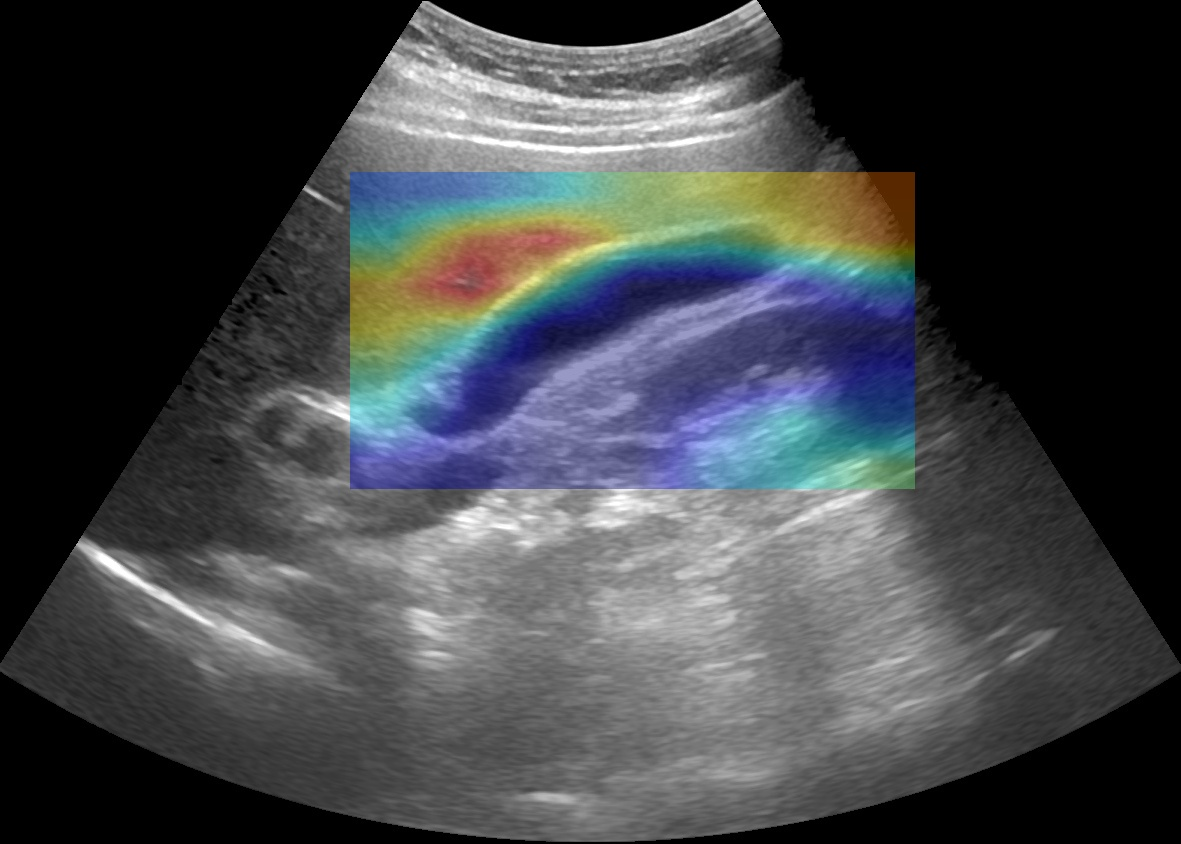
\includegraphics[width=\linewidth,height=8em]{figs/gbcnet/texture-1.jpg}
		\caption{}
		%\label{fig:multi-scale}
	\end{subfigure}
    \begin{subfigure}[b]{0.3\linewidth}
		\centering
		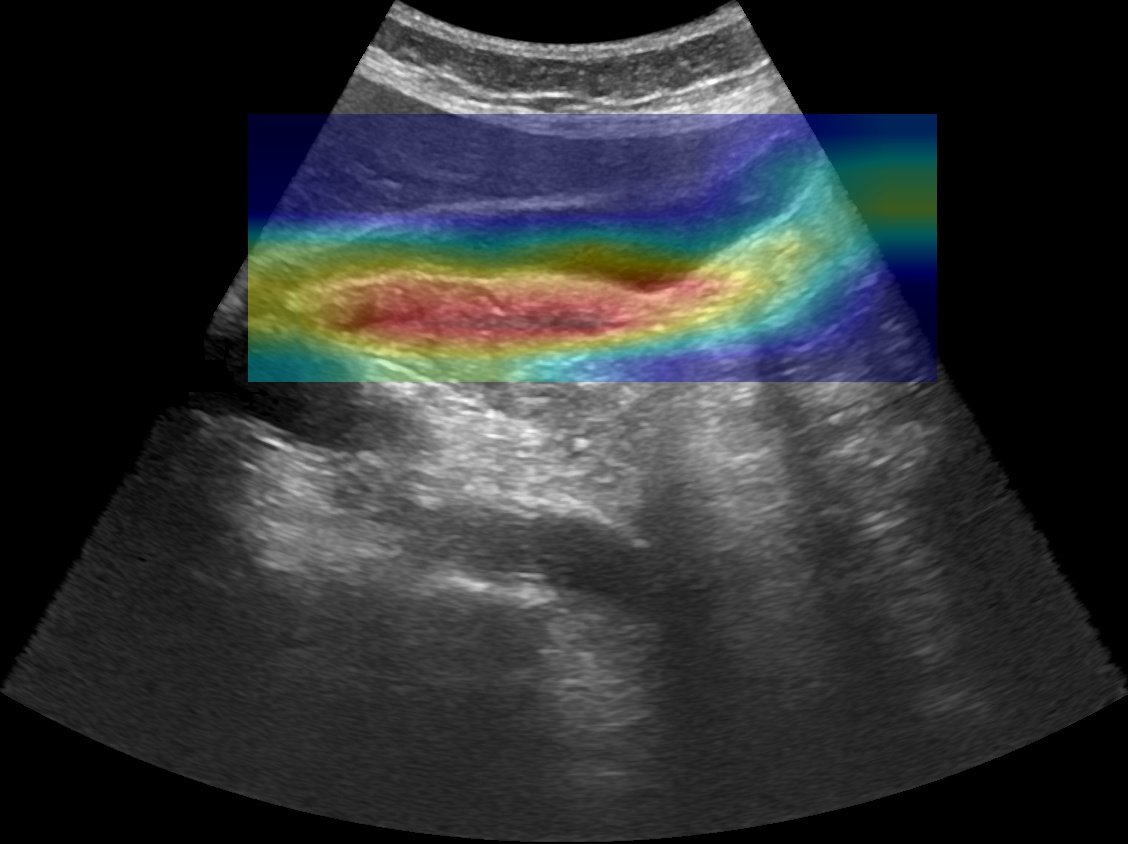
\includegraphics[width=\linewidth,height=8em]{figs/gbcnet/texture-2.jpg}
		\caption{}
		%\label{fig:multi-scale}
	\end{subfigure}
	\begin{subfigure}[b]{0.3\linewidth}
		\centering
		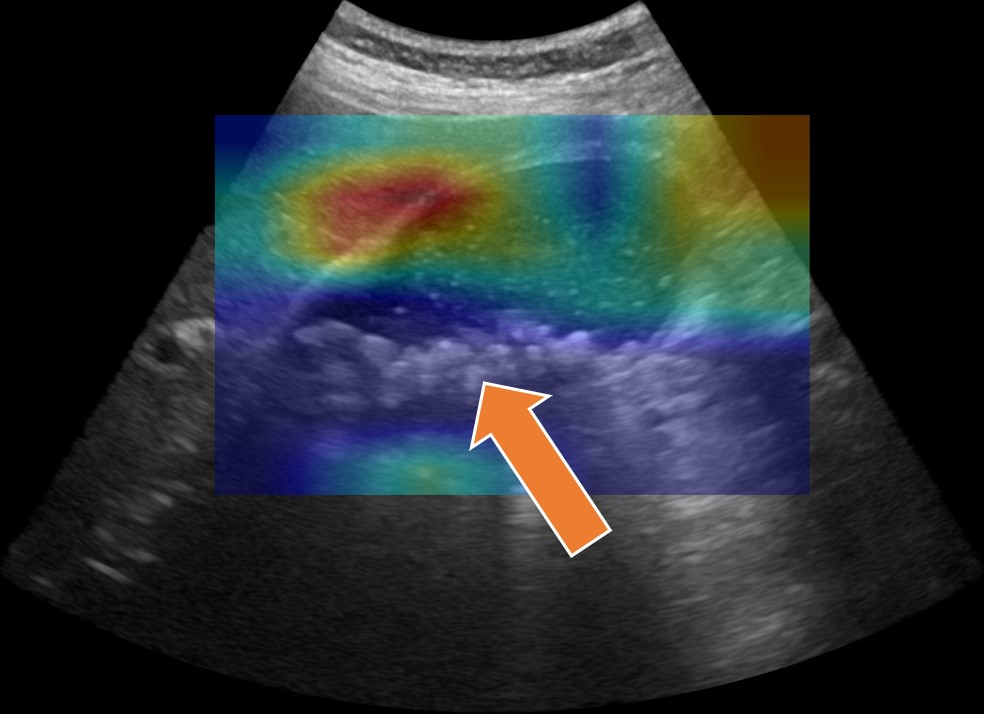
\includegraphics[width=\linewidth,height=8em]{figs/gbcnet/texture-3.jpg}
		\caption{}
		%\label{fig:multi-scale}
	\end{subfigure}
    \caption[Visualization of texture bias]{Grad-CAM visual of GBCNet trained without curriculum showing how the model tends to get biased due to the presence of textures due to noise or organ tissue. GBCNet focuses on - (a) adjacent liver tissues than the normal \gb, (b) the echogenic region below the \gb, and (c) liver textures instead of the stones (highlighted using the arrow).}
    \label{fig:texture_bias_sample}
\end{figure}
%
\begin{figure}[t]
	\centering
	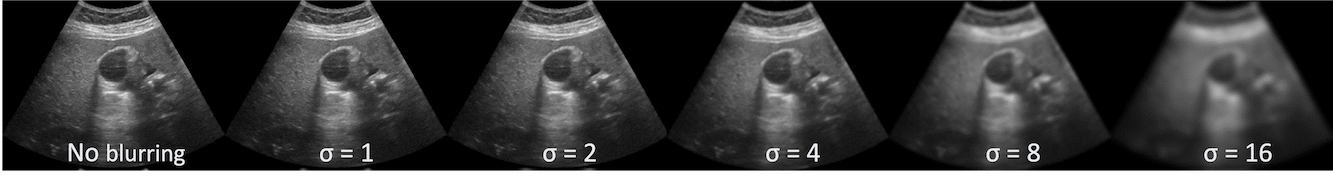
\includegraphics[width=0.95\linewidth]{figs/blur_sample_1.png}
	\caption[Gaussian blurring of USG data samples]{We simulate visual acuity through the Gaussian blur. Increasing $\sigma$ in a Gaussian filter decreases the visual acuity. Notice in the figure that, the effect of textures reduce as the visual acuity decreases and \gb shape and structure become more pronounced.}
	\label{fig:vis_acuity_sample}
\end{figure}

%% Curriculum
\subsection{Visual Acuity Inspired Curriculum}
%
We found that the textures having visual characteristics of soft tissue can adversely affect the performance of GBCNet (\cref{fig:texture_bias_sample}). We propose a curriculum to mitigate the texture bias and improve the classification. We observed that while the MS-SoP classifier is affected by texture bias, the region selection network still maintains a very high recall (\cref{tbl:perf_region}). Hence, we used the curriculum training only on the classifier and not on the region selection network.

\mypara{Visual Acuity in Humans}
%
Visual Acuity (VA) refers to the clarity and sharpness of human vision. Due to the immaturity of the retina and visual cortex, newborn children have very low VA \cite{courage1990visual}. The VA improves with the maturation of the retina and visual cortex. However, for children with congenital cataracts, the cortex matures despite the lenticular opacity. Such children begin their visual activity with higher initial VA. Evidence shows that children with high initial VA suffer to facilitate spatial analysis over expansive areas \cite{vogelsang2018VisualAcuity}.  Low VA renders blurry images that do not contain enough local information for the visual cortex to identify patterns. As a result, the visual cortex tries to increase the receptive field to facilitate spatial analysis over expansive areas and learn global features \cite{kwon2016compensation, smith2009smile}. 

\begin{algorithm}[t]
\small  
	\caption{Proposed Visual Acuity-based Curriculum}
	\label{va_algo}
	\SetAlgoLined
	\KwIn{$D^{\text{train}}$, Dataset of regions cropped from the original USG images.}
	\KwOut{Optimized model parameters $W^*$}
	Initialize $\sigma = \sigma_0$ \;
	%Set warm-up size to be $k'$ \;
	Initialize model parameters to $W$ \;
	
	\For {epoch=$\{1 \ldots, N\}$}{
		\eIf{$\sigma > 0$}{
		    $Z = \phi$ \;
    		\For {$x \in D^{\text{train}}$} {
    			$Z = Z \cup \{x \oast G(\sigma)\}$ \;
    		}
		    train($W, Z$)\;
		}
		{
		    train($W, D^{\text{train}}$) \;
		}
		\If{(epoch $> k'$) and (epoch$\%k == 0$)}{
			$\sigma = \lfloor \sigma/2 \rfloor$ \; 
		}
	}
\end{algorithm}


\mypara{Gaussian Blurring to Simulate Visual Acuity}
%
Gaussian filters are low-pass filters to cloak the high-frequency components of an input. A standard deviation $\sigma$ parameterizes the Gaussian filters. Increasing the $\sigma$ generates a higher amount of blur and low VA when convolved with an image. \cref{fig:vis_acuity_sample} shows how we can decrease the VA by increasing the $\sigma$ of a Gaussian filter. In our experiments, we have varied $\sigma$ from $1$ to $16$ to generate different levels of VA. 

\mypara{Proposed Curriculum}
%
While \cite{vogelsang2018VisualAcuity} demonstrates the improvement in receptive fields by gradually improving the sharpness of images during training, we take this observation further and show that the strategy of training on progressively higher resolution images also reduces the texture bias of a classification model. We propose a visual acuity-based training curriculum (\cref{va_algo}) that starts training the network with blurry and low-resolution \usg images and progressively increase the sharpness of training samples. The initial blurring allows the model to use an extended receptive field and focus on learning the global features such as the shape of the \gb while ignoring any noise or irrelevant textures. In the later phases, the sharp images allow the model to focus on the relevant local features in a controlled manner to make more accurate predictions. 

